
\documentclass[12pt]{letter}

\usepackage[margin=1in,footskip=0.25in]{geometry}
\usepackage{amsfonts}
\usepackage{pgf}
\usepackage{tikz}
\usepackage{amsmath}
\usepackage[latin1]{inputenc}
\usetikzlibrary{arrows,automata}
\usetikzlibrary{positioning}
\tikzset{>=latex}
\newcommand\tab[1][2cm]{\hspace*{#1}}

\begin{document}

Nov 12,2017 \\COMP.3040 Foundation of Computer Science \\ Viet Tran \\vtran1@cs.uml.edu

\centering Homework IV Solution

\flushleft

\begin{enumerate}

%	3.1	%
\item[\textbf{3.1)}]This exercise concerns TM M2, whose description and state diagram appear in Example 3.7. In each of the parts, give the sequence of configurations that M2 enters when started on the indicated input string.
\begin{enumerate}
	\item[\textbf{a}.] 0 \\
		$q_10,\sqcup q_2 \sqcup, \sqcup \sqcup q_{accept}.$ 

	\item[\textbf{c}.] 000 \\
		$q_100, \sqcup q_200, \sqcup $x$ q_3 0,\sqcup $x$0q_4\sqcup, \sqcup $x$0 \sqcup q_{reject}. $

	\item[\textbf{d}.] 000000 \\
		$q_1000000,\sqcup q_200 000,\sqcup $x$q_30 000, \sqcup $x$0 q_4 000, \sqcup $x0x$ q_300, \sqcup $x0x$ 0 q_4 0, \sqcup $x0x0x$q_3 \sqcup,\sqcup$x0x0x$q_3\sqcup,$
		$ \sqcup$x0x0$q_5$x$\sqcup,\sqcup$x0x$q_5$0x$\sqcup, \sqcup$x0$q_5$x0x$\sqcup,\sqcup$x$q_5$0x0x$\sqcup,\sqcup q_5$x0x0x$\sqcup, q_5\sqcup$x0x0x$\sqcup, \sqcup q_2$x0x0x$\sqcup,$
		$\sqcup$x$q_2$0x0x$\sqcup, \sqcup$xx$q_3$x0x$\sqcup,\sqcup$xxx$q_3$0x$\sqcup, \sqcup$xxx0$q_4$x$\sqcup,\sqcup$xxx0x$q_4\sqcup, \sqcup$xxx0x$\sqcup q_{reject}.$

	\item[\textbf{plus}.] 00000000 \\
		$q_1 0000 00, \sqcup q_2000 0000, \sqcup$x$q_3 00 0000, \sqcup$x$0 q_40 0000, \sqcup$x0x$q_30000, \sqcup$x0x0$q_4000, \sqcup$x0x0x$q_300,$
		$\sqcup$x0x0x0$q_40, \sqcup$x0x0x0x$q_3\sqcup, \sqcup$x0x0x0$q_5$x$\sqcup,\sqcup$x0x0x$q_5$0x$\sqcup, \sqcup$x0x0$q_5$x0x$\sqcup,\sqcup$x0x$q_5$0x0x$\sqcup,$
		$\sqcup$x0$q_5$x0x0x$\sqcup, \sqcup$x$q_5$0x0x0x$\sqcup, \sqcup q_5$x0x0x0x$\sqcup, q_5 \sqcup$x0x0x0x$\sqcup, \sqcup q_2$x0x0x0x$\sqcup, \sqcup$x$q_2$0x0x0x$\sqcup,$
		$\sqcup$xx$q_3$x0x0x$\sqcup, \sqcup$xxx$q_3$0x0x$\sqcup,\sqcup$xxx0$q_4$x0x$\sqcup, \sqcup$xxx0x$q_4$0x$\sqcup, \sqcup$xxx0xx$q_3$x$\sqcup, \sqcup$xxx0xxx$q_3\sqcup,$
		$\sqcup$xxx0xx$q_5$x$\sqcup,\sqcup$ xxx0x$q_5$xx$\sqcup, \sqcup$xxx0$q_5$xxx$\sqcup,\sqcup$xxx$q_5$0xxx$\sqcup, \sqcup$xx$q_5$x0xxx$\sqcup,$
		$\sqcup$x$q_5$xx0xxx$\sqcup,\sqcup q_5$xxx0xxx$\sqcup, q_5 \sqcup$xxx0xxx$\sqcup, \sqcup q_2$xxx0xxx$\sqcup,\sqcup$x$q_2$xx0xxx$\sqcup, \sqcup$xx$q_2$x0xxx$\sqcup,$
		$\sqcup$xxx$q_2$0xxx$\sqcup, \sqcup$xxxx$q_3$xxx$\sqcup,\sqcup$xxxxx$q_3$xx$\sqcup, \sqcup$xxxxxx$q_3$x$\sqcup,\sqcup$xxxxxxx$q_3 \sqcup, \sqcup$xxxxxx$q_5$x$\sqcup,$
		$\sqcup$xxxxx$q_5$xx$\sqcup,\sqcup$xxxx$q_5$xxx$\sqcup,\sqcup$xxx$q_5$xxxx$\sqcup,\sqcup$xx$q_5$xxxxx$\sqcup, \sqcup$x$q_5$xxxxxx$\sqcup,\sqcup q_5$xxxxxxx$\sqcup,$
		$q_5 \sqcup$xxxxxxx$\sqcup,\sqcup q_2$xxxxxxx$\sqcup,\sqcup$x$q_2$xxxxxx$\sqcup,\sqcup$xx$q_2$xxxxx$\sqcup, \sqcup$xxx$q_2$xxxx$\sqcup,\sqcup$xxxx$q_2$xxx$\sqcup,$
		$\sqcup$xxxxx$q_2$xx$\sqcup,\sqcup$xxxxxx$q_2$x$\sqcup,\sqcup$xxxxxxx$q_2\sqcup,\sqcup$xxxxxxx$\sqcup q_{accept}.$
\end{enumerate}

%	3.2	%
\item[\textbf{3.2)}]This exercise concerns TM M1, whose description and state diagram appear in Example 3.9. In each of the parts, give the sequence of configurations that M1 enters when started on the indicated input string.
\begin{enumerate}
	\item[\textbf{b}.] 1\#1. \\
	$q_1$1\#1 $\rightarrow$ x$q_3$\#1 $\rightarrow$ x\#$q_5$1 $\rightarrow$ x$q_6$\#x $\rightarrow$ $q_7$x\#x $\rightarrow$ x$q_1$\#x $\rightarrow$ x\#$q_8$x $\rightarrow$ x\#x$q_8\sqcup$ $\rightarrow$ x\#x$\sqcup q_{accept}.$

	\item[\textbf{c}.] 1\#\#1. \\
	$q_1$1\#\#1 $\rightarrow$ x$q_3$\#\#1 $\rightarrow$ x\#$q_5$\#1 $\rightarrow$ x\#\#$q_{reject}$1.

	\item[\textbf{d}.] 10\#11. \\
	$q_1$10\#11 $\rightarrow$ x$q_3$0\#11 $\rightarrow$ x0$q_3$\#11 $\rightarrow$ x0\#$q_5$11 $\rightarrow$ x0$q_6$\#x1 $\rightarrow$ x$q_7$0\#x1 $\rightarrow$ $q_7$x0\#x1 $\rightarrow$ x$q_1$0\#x1 $\rightarrow$ xx$q_2$\#x1 $\rightarrow$ xx\#$q_4$x1 $\rightarrow$ xx\#x$q_4$1 $\rightarrow$ xx\#x1$q_{reject} \sqcup.$

	\newpage

	\item[\textbf{e}.] 10\#10. \\
$q_1$10\#10 $\rightarrow$ x$q_3$0\#10 $\rightarrow$ x0$q_3$\#10 $\rightarrow$ x0\#$q_5$10 $\rightarrow$ x0$q_6$\#x0 $\rightarrow$ x$q_7$0\#x0 $\rightarrow$ $q_7$x0\#x0 $\rightarrow$ x$q_1$0\#x0 $\rightarrow$ xx$q_2$\#x0 $\rightarrow$ xx\#$q_4$x0 $\rightarrow$ xx\#x$q_4$0 $\rightarrow$ xx\#$q_6$xx $\rightarrow$ xx$q_6$\#xx $\rightarrow$ x$q_7$x\#xx $\rightarrow$ xx$q_1$\#xx $\rightarrow$ xx\#$q_8$xx $\rightarrow$ xx\#x$q_8$x $\rightarrow$ xx\#xx$q_8\sqcup \rightarrow$ xx\#xx$\sqcup q_{accept}.$

	\item[\textbf{plus}.] 01100\#01100. \\
	$q_1$01100\#01100 $\rightarrow$ x$q_2$1100\#01100 $\rightarrow$ x1$q_2$100\#01100 $\rightarrow$ x11$q_2$00\#01100 $\rightarrow$ x110$q_2$0\#01100 $\rightarrow$ x1100$q_2$\#01100 $\rightarrow$ x1100\#$q_4$01100 $\rightarrow$ x1100\#x$q_6$1100 $\rightarrow$ x1100\#$q_6$x1100 $\rightarrow$ x1100$q_6$\#x1100 $\rightarrow$ x110$q_7$0\#x1100 $\rightarrow$ x11$q_7$00\#x1100 $\rightarrow$ x1$q_7$100\#x1100 $\rightarrow$ x$q_7$1100\#x1100 $\rightarrow$ $q_7$x1100\#x1100 $\rightarrow$ x$q_1$1100\#x1100 $\rightarrow$ xx$q_3$100\#x1100 $\rightarrow$ xx1$q_3$00\#x1100 $\rightarrow$ xx10$q_3$0\#x1100 $\rightarrow$ xx100$q_3$\#x1100 $\rightarrow$ xx100\#$q_5$x1100 $\rightarrow$ xx100\#x$q_5$1100 $\rightarrow$ xx100\#$q_6$xx100 $\rightarrow$ xx100$q_6$\#xx100 $\rightarrow$ xx10$q_7$0\#xx100 $\rightarrow$ xx1$q_7$00\#xx100 $\rightarrow$ xx$q_7$100\#xx100 $\rightarrow$ x$q_7$x100\#xx100 $\rightarrow$ xx$q_1$100\#xx100 $\rightarrow$ xxx$q_3$00\#xx100 $\rightarrow$ xxx0$q_3$0\#xx100 $\rightarrow$ xxx00$q_3$\#xx100 $\rightarrow$ xxx00\#$q_5$xx100 $\rightarrow$ xxx00\#x$q_5$x100 $\rightarrow$ xxx00\#xx$q_5$100 $\rightarrow$ xxx00\#x$q_6$xx00 $\rightarrow$ xxx00\#$q_6$xxx00 $\rightarrow$ xxx00$q_6$\#xxx00 $\rightarrow$ xxx0$q_7$0\#xxx00 $\rightarrow$ xxx$q_7$00\#xxx00 $\rightarrow$ xx$q_7$x00\#xxx00 $\rightarrow$ xxx$q_1$00\#xxx00 $\rightarrow$ xxxx$q_2$0\#xxx00 $\rightarrow$ xxxx0$q_2$\#xxx00 $\rightarrow$ xxxx0\#$q_4$xxx00 $\rightarrow$ xxxx0\#x$q_4$xx00 $\rightarrow$ xxxx0\#xx$q_4$x00 $\rightarrow$ xxxx0\#xxx$q_4$00 $\rightarrow$ xxxx0\#xx$q_6$xx0 $\rightarrow$ xxxx0\#x$q_6$xxx0 $\rightarrow$ xxxx0\#$q_6$xxxx0 $\rightarrow$ xxxx0$q_6$\#xxxx0 $\rightarrow$ xxxx$q_7$0\#xxxx0 $\rightarrow$ xxx$q_7$x0\#xxxx0 $\rightarrow$ xxxx$q_1$0\#xxxx0 $\rightarrow$ xxxxx$q_2$\#xxxx0 $\rightarrow$ xxxxx\#$q_4$xxxx0 $\rightarrow$ xxxxx\#x$q_4$xxx0 $\rightarrow$ xxxxx\#xx$q_4$xx0 $\rightarrow$ xxxxx\#xxx$q_4$x0 $\rightarrow$ xxxxx\#xxxx$q_4$0 $\rightarrow$ xxxxx\#xxx$q_6$xx $\rightarrow$ xxxxx\#xx$q_6$xxx $\rightarrow$ xxxxx\#x$q_6$xxxx $\rightarrow$ xxxxx\#$q_6$xxxxx $\rightarrow$ xxxxx$q_6$\#xxxxx $\rightarrow$ xxxx$q_7$x\#xxxxx $\rightarrow$ xxxxx$q_1$\#xxxxx $\rightarrow$ xxxxx\#$q_8$xxxxx $\rightarrow$ xxxxx\#x$q_8$xxxx $\rightarrow$ xxxxx\#xx$q_8$xxx $\rightarrow$ xxxxx\#xxx$q_8$xx $\rightarrow$ xxxxx\#xxxx$q_8$x $\rightarrow$ xxxxx\#xxxxx$q_8$\textvisiblespace $\rightarrow$ 
xxxxx\#xxxxx $\sqcup q_{accept}\sqcup.$

	\item[\textbf{plus}.] 01101\#01100. \\
	$q_1$01101\#01100 $\rightarrow$ x$q_2$1101\#01100 $\rightarrow$ x1$q_2$101\#01100 $\rightarrow$ x11$q_2$01\#01100 $\rightarrow$ x110$q_2$1\#01100 $\rightarrow$ x1101$q_2$\#01100 $\rightarrow$ x1101\#$q_4$01100 $\rightarrow$ x1101\#x$q_6$1100 $\rightarrow$ x1101\#$q_6$x1100 $\rightarrow$ x1101$q_6$\#x1100 $\rightarrow$ x110$q_7$1\#x1100 $\rightarrow$ x11$q_7$01\#x1100 $\rightarrow$ x1$q_7$101\#x1100 $\rightarrow$ x$q_7$1101\#x1100 $\rightarrow$ $q_7$x1101\#x1100 $\rightarrow$ x$q_1$1101\#x1100 $\rightarrow$ xx$q_3$101\#x1100 $\rightarrow$ xx1$q_3$01\#x1100 $\rightarrow$ xx10$q_3$1\#x1100 $\rightarrow$ xx101$q_3$\#x1100 $\rightarrow$ xx101\#$q_5$x1100 $\rightarrow$ xx101\#x$q_5$1100 $\rightarrow$ xx101\#$q_6$xx100 $\rightarrow$ xx101$q_6$\#xx100 $\rightarrow$ xx10$q_7$1\#xx100 $\rightarrow$ xx1$q_7$01\#xx100 $\rightarrow$ xx$q_7$101\#xx100 $\rightarrow$ x$q_7$x101\#xx100 $\rightarrow$ xx$q_1$101\#xx100 $\rightarrow$ xxx$q_3$01\#xx100 $\rightarrow$ xxx0$q_3$1\#xx100 $\rightarrow$ xxx01$q_3$\#xx100 $\rightarrow$ xxx01\#$q_5$xx100 $\rightarrow$ xxx01\#x$q_5$x100 $\rightarrow$ xxx01\#xx$q_5$100 $\rightarrow$ xxx01\#x$q_6$xx00 $\rightarrow$ xxx01\#$q_6$xxx00 $\rightarrow$ xxx01$q_6$\#xxx00 $\rightarrow$ xxx0$q_7$1\#xxx00 $\rightarrow$ xxx$q_7$01\#xxx00 $\rightarrow$ xx$q_7$x01\#xxx00 $\rightarrow$ xxx$q_1$01\#xxx00 $\rightarrow$ xxxx$q_2$1\#xxx00 $\rightarrow$ xxxx1$q_2$\#xxx00 $\rightarrow$ xxxx1\#$q_4$xxx00 $\rightarrow$ xxxx1\#x$q_4$xx00 $\rightarrow$ xxxx1\#xx$q_4$x00 $\rightarrow$ xxxx1\#xxx$q_4$00 $\rightarrow$ xxxx1\#xx$q_6$xx0 $\rightarrow$ xxxx1\#x$q_6$xxx0 $\rightarrow$ xxxx1\#$q_6$xxxx0 $\rightarrow$ xxxx1$q_6$\#xxxx0 $\rightarrow$ xxxx$q_7$1\#xxxx0 $\rightarrow$ xxx$q_7$x1\#xxxx0 $\rightarrow$ xxxx$q_1$1\#xxxx0 $\rightarrow$ xxxxx$q_3$\#xxxx0 $\rightarrow$ xxxxx\#$q_5$xxxx0 $\rightarrow$ xxxxx\#x$q_5$xxx0 $\rightarrow$ xxxxx\#xx$q_5$xx0 $\rightarrow$ xxxxx\#xxx$q_5$x0 $\rightarrow$ xxxxx\#xxxx$q_5$0 $\rightarrow$ xxxxx\#xxxx0$q_{reject}\sqcup.$ 
\end{enumerate}

\leavevmode \\
%	3.8	%
\item[\textbf{3.8)}]Give implementation-level descriptions of Turing machines that decide the following languages over the alphabet \{0,1\}/ \\
\begin{enumerate}
	\item[\textbf{b}.] \{$w| w$ contains twice as many 0s as 1s\} \\
	\begin{enumerate}
		\item[\textbf{1.}] Begin scanning the tape for any unmarked 0s. Mark the first zero that is found. If there are no zeroes that have been marked, move the head back to the front of the tape and scan the tape for any unmarked 1s. If none are found, move to the accept state. Otherwise, move to reject state.
		\item[\textbf{2.}] Continue scanning the tape for the next unmarked 0. Mark it once found. If none are found, move to the reject state. Else, move the head back to the front of the tape.
		\item[\textbf{3.}] Begin scanning the tape for any unmarked 1s. Mark it once found. If none exist, move to the reject state. Else, move on to the next step.
		\item[\textbf{4.}] Move the head back to the beginning of the tape and restart scanning the tape for any unmarked 0s. Mark the next 0 that is found. If there are no zeroes that have been marked, move the head back to the front of the tape and scan for any unmarked 1s. If none are found, move to the accept state, otherwise move to the reject state.

State diagrams: \\ 
	\begin{center}
	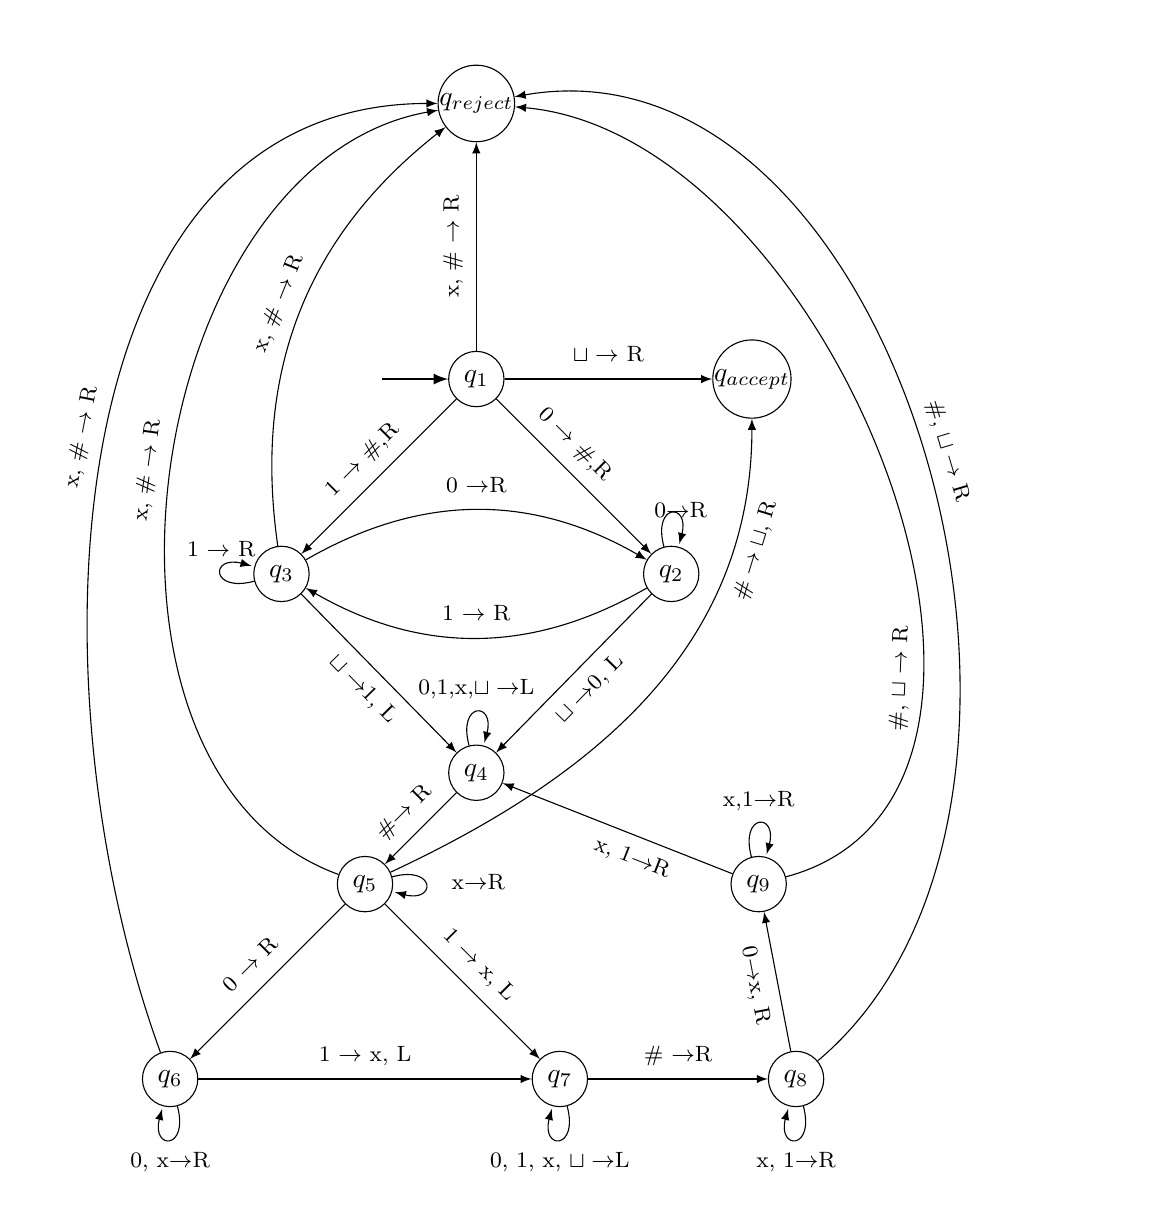
\begin{tikzpicture}[state/.style={circle, draw=black!100, inner sep=0pt, minimum size=20pt},node distance=3.5cm, on grid, auto] 
		\node[state] (q1) {$q_1$};
		\node[state] (q2) [below right=of q1] {$q_2$};
		\node[state] (q3) [below left=of q1] {$q_3$};
		\node[state] (q4) [below= 5cm of q1] {$q_4$};
		\node[state] (q5) [below left =2cm of q4] {$q_5$};
		\node[state] (q6) [below left= of q5] {$q_6$};
		\node[state] (q7) [below right= of q5] {$q_7$};
		\node[state] (q8) [right =3cm of q7] {$q_8$};
		\node[state] (q9) [right=5cm of q5] {$q_9$};
		\node[state] (qr) [above= of q1] {$q_{reject}$};
		\node[state] (qa) [right=3.5cm of q1] {$q_{accept}$};

		\draw[<-, thick] (q1) -- ++(-1.2cm,0);
		\path[->]
			(q1) edge node [midway, above, sloped, pos=0.4]{\footnotesize \begin{tabular}{c}0 $\rightarrow$ \#,R\end{tabular}} (q2)  edge node [midway, above, sloped]{\footnotesize \begin{tabular}{c}1 $\rightarrow$ \#,R\end{tabular}} (q3) edge node [midway, above, sloped]{\footnotesize \begin{tabular}{c}x, \# $\rightarrow$ R\end{tabular}} (qr) edge node [midway, above, sloped]{\footnotesize \begin{tabular}{c}$\sqcup \rightarrow$ R\end{tabular}} (qa) 
			
			(q2) edge [bend left] node [midway, above, sloped]{\footnotesize \begin{tabular}{c}1 $\rightarrow$ R\end{tabular}} (q3) edge node [midway, below, sloped]{\footnotesize \begin{tabular}{c}$\sqcup \rightarrow$0, L\end{tabular}} (q4)  edge [loop above] node [pos=0.9]{\footnotesize \begin{tabular}{c}0$\rightarrow$R\end{tabular}} (q2)

			(q3) edge [bend left] node [midway, above, sloped]{\footnotesize \begin{tabular}{c}0 $\rightarrow$R\end{tabular}} (q2) edge [loop left] node [midway, above]{\footnotesize \begin{tabular}{c}1 $\rightarrow$ R\end{tabular}} (q3)  edge [bend left] node [midway, above, sloped ]{\footnotesize \begin{tabular}{c}x, \# $\rightarrow$ R\end{tabular}} (qr) edge node [midway, below, sloped]{\footnotesize \begin{tabular}{c}$\sqcup \rightarrow$1, L\end{tabular}} (q4) 

			(q4) edge node [midway, above, sloped]{\footnotesize \begin{tabular}{c} \#$\rightarrow$ R\end{tabular}} (q5)  edge [loop above] node [midway, above]{\footnotesize \begin{tabular}{c}0,1,x,$\sqcup\rightarrow$L\end{tabular}} (q4) 
			
			(q5) edge [loop right] node{\footnotesize \begin{tabular}{c}x$\rightarrow$R\end{tabular}} (q5) edge [out=160,in=190] node [midway, above, sloped]{\footnotesize \begin{tabular}{c}x, \# $\rightarrow$ R\end{tabular}} (qr) edge node [midway, above, sloped]{\footnotesize \begin{tabular}{c}0 $\rightarrow$ R\end{tabular}} (q6) edge node [midway, above, sloped]{\footnotesize \begin{tabular}{c}1 $\rightarrow$ x, L\end{tabular}} (q7) edge [out=25,in=270] node [midway, below, sloped, pos=0.8]{\footnotesize \begin{tabular}{c}$ \#\rightarrow\sqcup,$ R\end{tabular}} (qa) 
	
			(q6) edge [loop below] node [midway, below] {\footnotesize \begin{tabular}{c}0, x$\rightarrow$R\end{tabular}} (q6)  edge node [midway, above, sloped]{\footnotesize \begin{tabular}{c}1 $\rightarrow$ x, L\end{tabular}} (q7) edge [out=110,in=180] node [midway, above, sloped]{\footnotesize \begin{tabular}{c}x, \# $\rightarrow$ R\end{tabular}} (qr)

			(q7) edge [loop below] node [midway, below] {\footnotesize \begin{tabular}{c}0, 1, x, $\sqcup \rightarrow$L\end{tabular}} (q7)  edge node [midway, above, sloped]{\footnotesize \begin{tabular}{c}\# $\rightarrow$R\end{tabular}} (q8)

			(q8) edge [loop below] node [midway, below] {\footnotesize \begin{tabular}{c}x, 1$\rightarrow$R\end{tabular}} (q8) edge node [midway, below, sloped] {\footnotesize \begin{tabular}{c}0$\rightarrow$x, R\end{tabular}} (q9) edge [out=40,in=10] node [midway, above, sloped]{\footnotesize \begin{tabular}{c}\#, $\sqcup \rightarrow$ R\end{tabular}} (qr)

			(q9) edge node [midway, below, sloped,pos=0.4] {\footnotesize \begin{tabular}{c}x, 1$\rightarrow$R\end{tabular}} (q4) edge [out=15,in=355] node [midway, above, sloped, pos=0.3]{\footnotesize \begin{tabular}{c}\#, $\sqcup \rightarrow$ R\end{tabular}} (qr) edge [loop above] node [midway, above] {\footnotesize \begin{tabular}{c}x,1$ \rightarrow$R\end{tabular}} (q9) 
			;
	\end{tikzpicture}
	\end{center}
		
	\item[\textbf{plus}.] 010100 \\
		$q_1$010100 $\rightarrow$ $\#$$q_2$10100 $\rightarrow$ $\#$0$q_3$0100 $\rightarrow$ $\#$01$q_2$100 $\rightarrow$ $\#$010$q_3$00 $\rightarrow$ $\#$0101$q_2$0\\
		$\rightarrow$ $\#$01010$q_2$$\sqcup$ $\rightarrow$ $\#$0101$q_4$00 $\rightarrow$ $\#$010$q_4$100 $\rightarrow$ $\#$01$q_4$0100 $\rightarrow$ $\#$0$q_4$10100 \\
		$\rightarrow$ $\#$$q_4$010100 $\rightarrow$ $q_4$$\#$010100 $\rightarrow$ $\#$$q_5$010100 $\rightarrow$ $\#$0$q_6$10100 $\rightarrow$ $\#$$q_7$0$x$0100 \\
		$\rightarrow$ $q_7$$\#$0$x$0100 $\rightarrow$ $\#$$q_8$0$x$0100 $\rightarrow$ $\#$$x$$q_9$$x$0100 $\rightarrow$ $\#$$xx$$q_9$0100 $\rightarrow$ $\#$$x$$q_4$$xx$100\\
		$\rightarrow$ $\#$$q_4$$xxx$100 $\rightarrow$ $q_4$$\#$$xxx$100 $\rightarrow$ $\#$$q_5$$xxx$100 $\rightarrow$ $\#$$x$$q_5$$xx$100 $\rightarrow$ $\#$$xx$$q_5$$x$100 \\
		$\rightarrow$ $\#$$xxx$$q_5$100 $\rightarrow$ $\#$$xx$$q_7$$xx$00 $\rightarrow$ $\#$$x$$q_7$$xxx$00 $\rightarrow$ $\#$$q_7$$xxxx$00 $\rightarrow$ $q_7$$\#$$xxxx$00 $\rightarrow$ $\#$$q_8$$xxxx$00 $\rightarrow$ $\#$$x$$q_8$$xxx$00 $\rightarrow$ $\#$$xx$$q_8$$xx$00 $\rightarrow$ $\#$$xxx$$q_8$$x$00 $\rightarrow$ $\#$$xxxx$$q_8$00 \\
		$\rightarrow$ $\#$$xxxxx$$q_9$0 $\rightarrow$ $\#$$xxxx$$q_4$$xx$ $\rightarrow$ $\#$$xxx$$q_4$$xxx$ $\rightarrow$ $\#$$xx$$q_4$$xxxx$ $\rightarrow$ $\#$$x$$q_4$$xxxxx$ $\rightarrow$ $\#$$q_4$$xxxxxx$ $\rightarrow$ $q_4$$\#$$xxxxxx$ $\rightarrow$ $\#$$q_5$$xxxxxx$ $\rightarrow$ $\#$$x$$q_5$$xxxxx$ $\rightarrow$ $\#$$xx$$q_5$$xxxx$ \\
		$\rightarrow$ $\#$$xxx$$q_5$$xxx$ $\rightarrow$ $\#$$xxxx$$q_5$$xx$ $\rightarrow$ $\#$$xxxxx$$q_5$$x$ $\rightarrow$ $\#$$xxxxxx$$q_5$$\sqcup$ $\rightarrow$ $\#$$xxxxxx$$\sqcup$$q_{accept}$\\
		
	\item[\textbf{plus}.] 010101 \\
		$q_1$010101 $\rightarrow$ $\#$$q_2$10101 $\rightarrow$ $\#$0$q_3$0101 $\rightarrow$ $\#$01$q_2$101 $\rightarrow$ $\#$0101$q_3$01 $\rightarrow$ $\#$0101$q_2$1\\
		$\rightarrow$ $\#$01010$q_3$$\sqcup$ $\rightarrow$ $\#$0101$q_4$01 $\rightarrow$ $\#$010$q_4$101 $\rightarrow$ $\#$01$q_4$0101 $\rightarrow$ $\#$0$q_4$10101 \\
		$\rightarrow$ $\#$$q_4$010101 $\rightarrow$ $q_4$$\#$010101 $\rightarrow$ $\#$$q_5$010101 $\rightarrow$ $\#$0$q_6$10101 $\rightarrow$ $\#$$q_7$0$x$0101 \\
		$\rightarrow$ $q_7$$\#$0$x$0101 $\rightarrow$ $\#$$q_8$0$x$0101 $\rightarrow$ $\#$$x$$q_9$$x$0101 $\rightarrow$ $\#$$xx$$q_9$0101 $\rightarrow$ $\#$$x$$q_4$$xx$101\\
		 $\rightarrow$ $\#$$q_4$$xxx$101 $\rightarrow$ $q_4$$\#$$xxx$101 $\rightarrow$ $\#$$q_5$$xxx$101 $\rightarrow$ $\#$$x$$q_5$$xx$101 $\rightarrow$ $\#$$xx$$q_5$$x$101\\
		  $\rightarrow$ $\#$$xxx$$q_5$101 $\rightarrow$ $\#$$xx$$q_7$$xx$01 $\rightarrow$ $\#$$x$$q_7$$xxx$01 $\rightarrow$ $\#$$q_7$$xxxx$01 $\rightarrow$ $q_7$$\#$$xxxx$01 \\
		  $\rightarrow$ $\#$$q_8$$xxxx$01 $\rightarrow$ $\#$$x$$q_8$$xxx$01 $\rightarrow$ $\#$$xx$$q_8$$xx$01 $\rightarrow$ $\#$$xxx$$q_8$$x$01 $\rightarrow$ $\#$$xxxx$$q_8$01 \\
		  $\rightarrow$ $\#$$xxxxx$$q_9$1 $\rightarrow$ $\#$$xxxxx$1$q_9$$\sqcup$ $\rightarrow$ $\#$$xxxxx$1$\sqcup$$q_{reject}$\\
	\end{enumerate}

	\item[\textbf{c}.] \{$w| w$ does not contain twice as many 0s as 1s\} \\
	\begin{enumerate}
		\item[\textbf{1.}] Begin scanning the tape for any unmarked 0s. Mark the first zero that is found. of there are no unmarked zeroes, move the head back to the front of the tape and re scan for unmarked zeroes.
		\item[\textbf{2.}] Mark the next unmarked zero. If there are none, move to the accept state. Else, move the head back to the front of the tape. 
		\item[\textbf{3.}] Scan the tape for 1s and mark the first one that is found. If there are no 1s that have been marked, move to the accept state.
		\item[\textbf{4.}] Move the head to the start of the tape and scan again for any unmarked 0s. If there are none, move on to step 2.
		\item[\textbf{5.}] Move the head to the start of the tape again to scan for any unmarked 1s. If there are none, move to the reject state. Else, move to the accept state. 

State diagrams: \\ 
	\begin{center}
	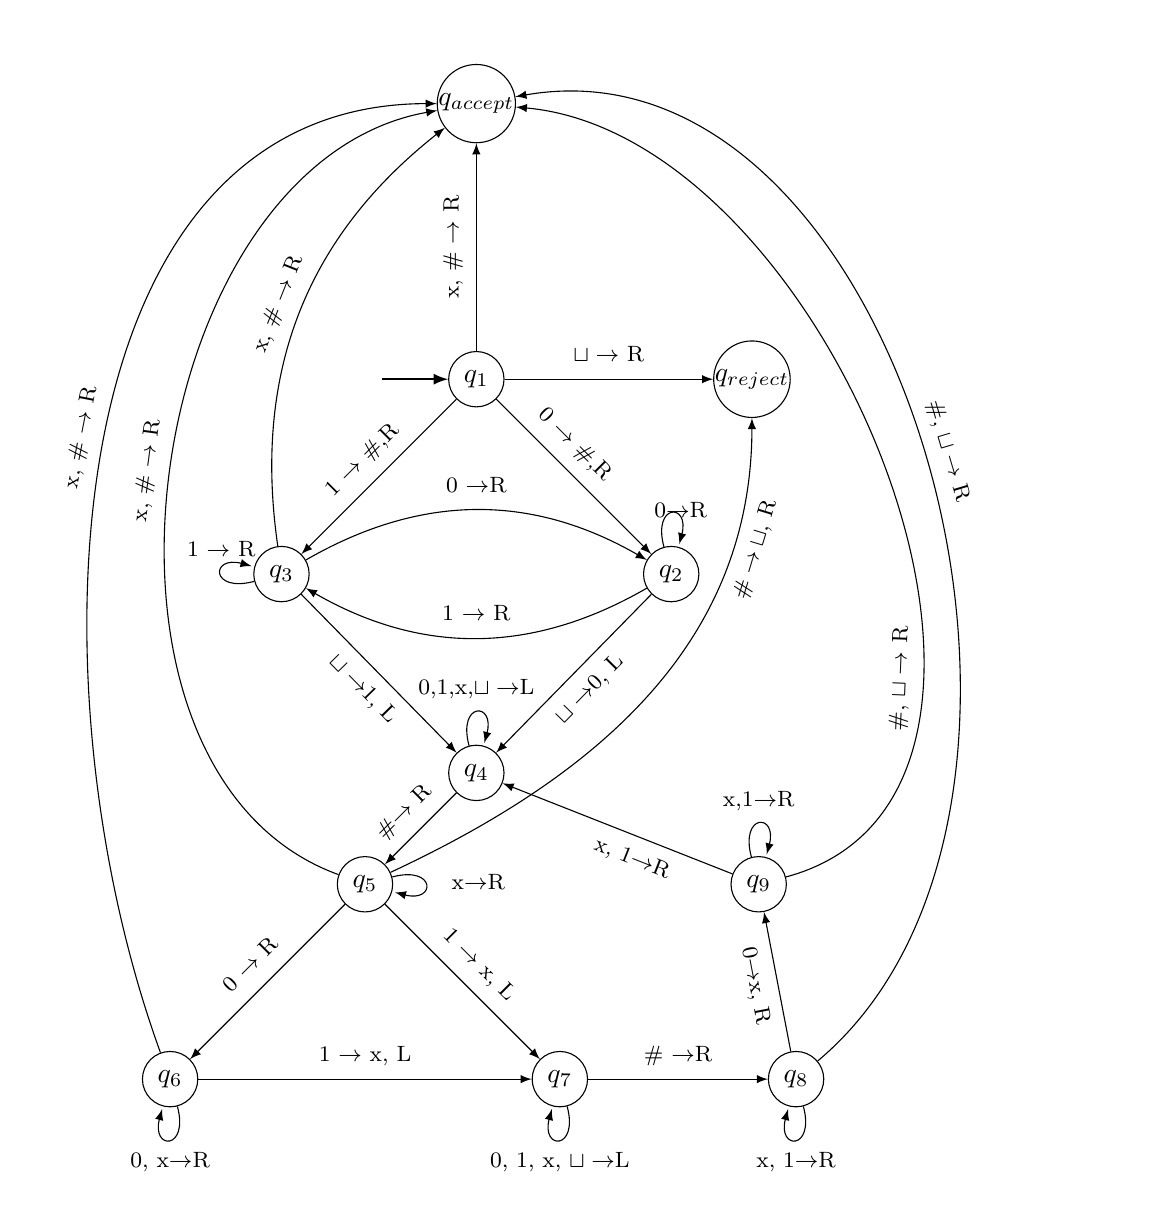
\begin{tikzpicture}[state/.style={circle, draw=black!100, inner sep=0pt, minimum size=20pt},node distance=3.5cm, on grid, auto] 
		\node[state] (q1) {$q_1$};
		\node[state] (q2) [below right=of q1] {$q_2$};
		\node[state] (q3) [below left=of q1] {$q_3$};
		\node[state] (q4) [below= 5cm of q1] {$q_4$};
		\node[state] (q5) [below left =2cm of q4] {$q_5$};
		\node[state] (q6) [below left= of q5] {$q_6$};
		\node[state] (q7) [below right= of q5] {$q_7$};
		\node[state] (q8) [right =3cm of q7] {$q_8$};
		\node[state] (q9) [right=5cm of q5] {$q_9$};
		\node[state] (qr) [above= of q1] {$q_{accept}$};
		\node[state] (qa) [right=3.5cm of q1] {$q_{reject}$};

		\draw[<-, thick] (q1) -- ++(-1.2cm,0);
		\path[->]
			(q1) edge node [midway, above, sloped, pos=0.4]{\footnotesize \begin{tabular}{c}0 $\rightarrow$ \#,R\end{tabular}} (q2)  edge node [midway, above, sloped]{\footnotesize \begin{tabular}{c}1 $\rightarrow$ \#,R\end{tabular}} (q3) edge node [midway, above, sloped]{\footnotesize \begin{tabular}{c}x, \# $\rightarrow$ R\end{tabular}} (qr) edge node [midway, above, sloped]{\footnotesize \begin{tabular}{c}$\sqcup \rightarrow$ R\end{tabular}} (qa) 
			
			(q2) edge [bend left] node [midway, above, sloped]{\footnotesize \begin{tabular}{c}1 $\rightarrow$ R\end{tabular}} (q3) edge node [midway, below, sloped]{\footnotesize \begin{tabular}{c}$\sqcup \rightarrow$0, L\end{tabular}} (q4)  edge [loop above] node [pos=0.9]{\footnotesize \begin{tabular}{c}0$\rightarrow$R\end{tabular}} (q2)

			(q3) edge [bend left] node [midway, above, sloped]{\footnotesize \begin{tabular}{c}0 $\rightarrow$R\end{tabular}} (q2) edge [loop left] node [midway, above]{\footnotesize \begin{tabular}{c}1 $\rightarrow$ R\end{tabular}} (q3)  edge [bend left] node [midway, above, sloped ]{\footnotesize \begin{tabular}{c}x, \# $\rightarrow$ R\end{tabular}} (qr) edge node [midway, below, sloped]{\footnotesize \begin{tabular}{c}$\sqcup \rightarrow$1, L\end{tabular}} (q4) 

			(q4) edge node [midway, above, sloped]{\footnotesize \begin{tabular}{c} \#$\rightarrow$ R\end{tabular}} (q5)  edge [loop above] node [midway, above]{\footnotesize \begin{tabular}{c}0,1,x,$\sqcup\rightarrow$L\end{tabular}} (q4) 
			
			(q5) edge [loop right] node{\footnotesize \begin{tabular}{c}x$\rightarrow$R\end{tabular}} (q5) edge [out=160,in=190] node [midway, above, sloped]{\footnotesize \begin{tabular}{c}x, \# $\rightarrow$ R\end{tabular}} (qr) edge node [midway, above, sloped]{\footnotesize \begin{tabular}{c}0 $\rightarrow$ R\end{tabular}} (q6) edge node [midway, above, sloped]{\footnotesize \begin{tabular}{c}1 $\rightarrow$ x, L\end{tabular}} (q7) edge [out=25,in=270] node [midway, below, sloped, pos=0.8]{\footnotesize \begin{tabular}{c}$ \#\rightarrow\sqcup,$ R\end{tabular}} (qa) 
	
			(q6) edge [loop below] node [midway, below] {\footnotesize \begin{tabular}{c}0, x$\rightarrow$R\end{tabular}} (q6)  edge node [midway, above, sloped]{\footnotesize \begin{tabular}{c}1 $\rightarrow$ x, L\end{tabular}} (q7) edge [out=110,in=180] node [midway, above, sloped]{\footnotesize \begin{tabular}{c}x, \# $\rightarrow$ R\end{tabular}} (qr)

			(q7) edge [loop below] node [midway, below] {\footnotesize \begin{tabular}{c}0, 1, x, $\sqcup \rightarrow$L\end{tabular}} (q7)  edge node [midway, above, sloped]{\footnotesize \begin{tabular}{c}\# $\rightarrow$R\end{tabular}} (q8)

			(q8) edge [loop below] node [midway, below] {\footnotesize \begin{tabular}{c}x, 1$\rightarrow$R\end{tabular}} (q8) edge node [midway, below, sloped] {\footnotesize \begin{tabular}{c}0$\rightarrow$x, R\end{tabular}} (q9) edge [out=40,in=10] node [midway, above, sloped]{\footnotesize \begin{tabular}{c}\#, $\sqcup \rightarrow$ R\end{tabular}} (qr)

			(q9) edge node [midway, below, sloped,pos=0.4] {\footnotesize \begin{tabular}{c}x, 1$\rightarrow$R\end{tabular}} (q4) edge [out=15,in=355] node [midway, above, sloped, pos=0.3]{\footnotesize \begin{tabular}{c}\#, $\sqcup \rightarrow$ R\end{tabular}} (qr) edge [loop above] node [midway, above] {\footnotesize \begin{tabular}{c}x,1$ \rightarrow$R\end{tabular}} (q9) 
			;
	\end{tikzpicture}
	\end{center}

	\item[\textbf{plus}.] 000111 \\

$q_1$000111 $\rightarrow$ $\#$$q_2$00111 $\rightarrow$ $\#$0$q_2$00111 $\rightarrow$ $\#$00$q_2$0111 $\rightarrow$ $\#$000$q_2$111\\
		$\rightarrow$ $\#$0000$q_3$11 $\rightarrow$ $\#$00001$q_3$1 $\rightarrow$ $\#$00001$q_4$11 $\rightarrow$ $\#$0000$q_4$111 $\rightarrow$ $\#$000$q_4$0111 \\
		$\rightarrow$ $\#$00$q_4$00111 $\rightarrow$ $\#$0$q_4$000111 $\rightarrow$ $\#$$q_4$0000111 $\rightarrow$ $q_4$$\#$0000111 $\rightarrow$ $\#$$q_5$0000111 \\
		$\rightarrow$ $\#$0$q_6$000111 $\rightarrow$ $\#$00$q_6$00111 $\rightarrow$ $\#$000$q_6$0111 $\rightarrow$ $\#$0000$q_6$111 $\rightarrow$ $\#$000$q_7$0$x$11 \\
		$\rightarrow$ $\#$00$q_7$00$x$11 $\rightarrow$ $\#$0$q_7$000$x$11 $\rightarrow$ $\#$$q_7$0000$x$11 $\rightarrow$ $q_7$$\#$0000$x$11 $\rightarrow$ $\#$$q_8$0000$x$11 \\
		$\rightarrow$ $\#$$x$$q_9$000$x$11 $\rightarrow$ $\#$$q_4$$xx$00$x$11 $\rightarrow$ $q_4$$\#$$xx$00$x$11 $\rightarrow$ $\#$$q_5$$xx$00$x$11 $\rightarrow$ $\#$$x$$q_5$$x$00$x$11 \\
		$\rightarrow$ $\#$$xx$$q_5$00$x$11 $\rightarrow$ $\#$$xx$0$q_6$0$x$11 $\rightarrow$ $\#$$xx$00$q_6$$x$11 $\rightarrow$ $\#$$xx$00$x$$q_6$11 $\rightarrow$ $\#$$xx$00$q_7$$xx$1 \\
		$\rightarrow$ $\#$$xx$0$q_7$0$xx$1 $\rightarrow$ $\#$$xx$$q_7$00$xx$1 $\rightarrow$ $\#$$x$$q_7$$x$00$xx$1 $\rightarrow$ $\#$$q_7$$xx$00$xx$1 $\rightarrow$ $q_7$$\#$$xx$00$xx$1 \\
		$\rightarrow$ $\#$$q_8$$xx$00$xx$1 $\rightarrow$ $\#$$x$$q_8$$x$00$xx$1 $\rightarrow$ $\#$$xx$$q_8$00$xx$1 $\rightarrow$ $\#$$xxx$$q_9$0$xx$1 $\rightarrow$ $\#$$xx$$q_4$$xxxx$1 \\
		$\rightarrow$ $\#$$x$$q_4$$xxxxx$1 $\rightarrow$ $\#$$q_4$$xxxxxx$1 $\rightarrow$ $q_4$$\#$$xxxxxx$1 $\rightarrow$ $\#$$q_5$$xxxxxx$1 $\rightarrow$ $\#$$x$$q_5$$xxxxx$1 \\
		$\rightarrow$ $\#$$xx$$q_5$$xxxx$1 $\rightarrow$ $\#$$xxx$$q_5$$xxx$1 $\rightarrow$ $\#$$xxxx$$q_5$$xx$1 $\rightarrow$ $\#$$xxxxx$$q_5$$x$1 $\rightarrow$ $\#$$xxxxxx$$q_5$1 \\
		$\rightarrow$ $\#$$xxxxx$$q_7$$xx$ $\rightarrow$ $\#$$xxxx$$q_7$$xxx$ $\rightarrow$ $\#$$xxx$$q_7$$xxxx$ $\rightarrow$ $\#$$xx$$q_7$$xxxxx$ $\rightarrow$ $\#$$x$$q_7$$xxxxxx$ \\
		$\rightarrow$ $\#$$q_7$$xxxxxxx$ $\rightarrow$ $q_7$$\#$$xxxxxxx$ $\rightarrow$ $\#$$q_8$$xxxxxxx$ $\rightarrow$ $\#$$x$$q_8$$xxxxxx$ $\rightarrow$ $\#$$xx$$q_8$$xxxxx$ \\
		$\rightarrow$ $\#$$xxx$$q_8$$xxxx$ $\rightarrow$ $\#$$xxxx$$q_8$$xxx$ $\rightarrow$ $\#$$xxxxx$$q_8$$xx$ $\rightarrow$ $\#$$xxxxxx$$q_8$$x$ $\rightarrow$ $\#$$xxxxxxx$$q_8$$\sqcup$\\
		$\rightarrow$ $\#$$xxxxxxx$$\sqcup$$q_{accept}$\\

	\item[\textbf{plus}.] 000110 \\

		$q_1$000110 $\rightarrow$ $\#$$q_2$00110 $\rightarrow$ $\#$0$q_2$0110 $\rightarrow$ $\#$00$q_2$110 $\rightarrow$ $\#$000$q_3$10 $\rightarrow$ $\#$00011$q_2$$\sqcup$ \\
		$\rightarrow$ $\#$0001$q_4$10 $\rightarrow$ $\#$000$q_4$110 $\rightarrow$ $\#$00$q_4$0110 $\rightarrow$ $\#$0$q_4$00110 $\rightarrow$ $\#$$q_4$000110 \\
		$\rightarrow$ $q_4$$\#$000110 $\rightarrow$ $\#$$q_5$000110 $\rightarrow$ $\#$0$q_5$00110 $\rightarrow$ $\#$00$q_5$0110 $\rightarrow$ $\#$000$q_5$110 \\
		$\rightarrow$ $\#$000$q_5$110 $\rightarrow$ $\#$00$q_7$0$x$10 $\rightarrow$ $\#$0$q_7$00$x$10 $\rightarrow$ $\#$$q_7$000$x$10 $\rightarrow$ $q_7$$\#$000$x$10 \\
		$\rightarrow$ $\#$$q_8$000$x$10 $\rightarrow$ $\#$$x$$q_9$00$x$10 $\rightarrow$ $\#$$q_4$$xx$0$x$10 $\rightarrow$ $q_4$$\#$$xx$0$x$10 $\rightarrow$ $\#$$q_5$$xx$0$x$10 \\
		$\rightarrow$ $\#$$x$$q_5$$x$0$x$10 $\rightarrow$ $\#$$xx$$q_5$0$x$10 $\rightarrow$ $\#$$xx$0$q_6$$x$10 $\rightarrow$ $\#$$xx$0$x$$q_6$10 $\rightarrow$ $\#$$xx$0$q_7$$xx$0 \\
		$\rightarrow$ $\#$$xx$$q_7$0$xx$0 $\rightarrow$ $\#$$x$$q_7$$x$0$xx$0 $\rightarrow$ $\#$$q_7$$xx$0$xx$0 $\rightarrow$ $q_7$$\#$$xx$0$xx$0 $\rightarrow$ $\#$$q_8$$xx$0$xx$0 \\
		$\rightarrow$ $\#$$x$$q_8$$x$0$xx$0 $\rightarrow$ $\#$$xx$$q_8$0$xx$0 $\rightarrow$ $\#$$xxx$$q_9$$xx$0 $\rightarrow$ $\#$$xxx$$x$$q_9$$x$0 $\rightarrow$ $\#$$xxx$$xx$$q_9$0 \\
		$\rightarrow$ $\#$$xxxx$$q_4$$xx$ $\rightarrow$ $\#$$xxx$$q_4$$x$$xx$ $\rightarrow$ $\#$$xx$$q_4$$xxxx$ $\rightarrow$ $\#$$x$$q_4$$xxxxx$ $\rightarrow$ $\#$$q_4$$xxxxxx$ \\
		$\rightarrow$ $q_4$$\#$$xxxxxx$ $\rightarrow$ $\#$$q_5$$xxxxxx$ $\rightarrow$ $\#$$x$$q_5$$xxxxx$ $\rightarrow$ $\#$$xx$$q_5$$xxxx$ $\rightarrow$ $\#$$xxx$$q_5$$xxx$ \\
		$\rightarrow$ $\#$$xxxx$$q_5$$xx$ $\rightarrow$ $\#$$xxxxx$$q_5$$x$  $\rightarrow$ $\#$$xxxxxx$$q_5$$\sqcup$ $\rightarrow$ $\#$$xxxxxx$$\sqcup$$q_{reject}$ 

	\end{enumerate}

\item[\textbf{Modified M2}:]
	\leavevmode \\
	\begin{enumerate}
		\item[\textbf{b}.] To recognize odd numbers of 0s
		\leavevmode \\
		\begin{center}
		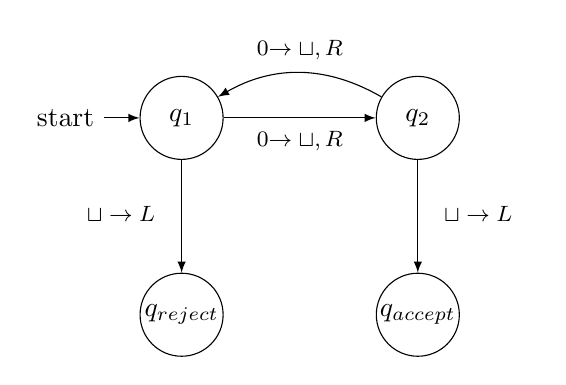
\begin{tikzpicture}[state/.style={circle, draw=black!100, inner sep=0pt, minimum size=30pt},node distance=3cm, on grid, auto] 
		\node[state,initial] (q1) {$q_1$};
		\node[state] (q2) [right=of q1] {$q_2$};
		\node[state] (qr) [below=2.5cm of q1] {$q_{reject}$};
		\node[state] (qa) [below=2.5cm of q2] {$q_{accept}$};

		\path[->]
			(q1) edge node [midway, below] {\footnotesize \begin{tabular}{c}0$\rightarrow\sqcup ,R$\end{tabular}} (q2) edge node [left] {\footnotesize \begin{tabular}{c}$\sqcup \rightarrow L$\end{tabular}} (qr)
			(q2) edge [bend right] node [midway, above] {\footnotesize \begin{tabular}{c}0$\rightarrow\sqcup,R$\end{tabular}} (q1)  edge node {\footnotesize \begin{tabular}{c}$\sqcup \rightarrow L$\end{tabular}} (qa);
		\end{tikzpicture}
		\end{center}
		000 \\
		$q_1$000 $\rightarrow$ $\sqcup$$q_2$00 $\rightarrow$ $\sqcup$$\sqcup$$q_1$0 $\rightarrow$ $\sqcup$$\sqcup$$\sqcup$$q_2$$\sqcup$ $\rightarrow$ $\sqcup$$\sqcup$$q_{accept}$$\sqcup$$\sqcup$\\
		\leavevmode \\
		0000\\
		$q_1$0000 $\rightarrow$ $\sqcup$$q_2$000 $\rightarrow$ $\sqcup$$\sqcup$$q_1$00 $\rightarrow$ $\sqcup$$\sqcup$$\sqcup$$q_2$0 $\rightarrow$ $\sqcup$$\sqcup$$\sqcup$$\sqcup$$q_1$$\sqcup$ $\rightarrow$ $\sqcup$$\sqcup$$\sqcup$$q_{reject}$$\sqcup$
		
		\item[\textbf{c}.] To recognize even numbers of 0s
		\leavevmode \\
		\begin{center}
		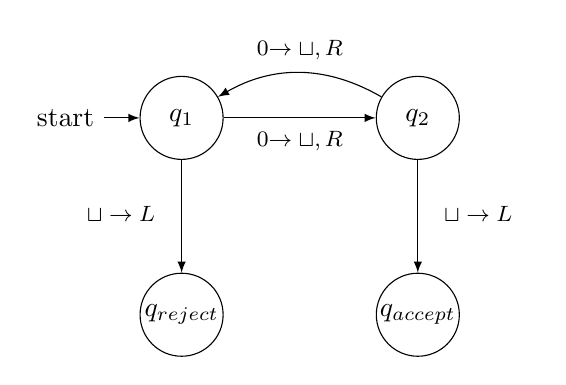
\begin{tikzpicture}[state/.style={circle, draw=black!100, inner sep=0pt, minimum size=30pt},node distance=3cm, on grid, auto] 
		\node[state,initial] (q1) {$q_1$};
		\node[state] (q2) [right=of q1] {$q_2$};
		\node[state] (qr) [below=2.5cm of q1] {$q_{reject}$};
		\node[state] (qa) [below=2.5cm of q2] {$q_{accept}$};

		\path[->]
			(q1) edge node [midway, below] {\footnotesize \begin{tabular}{c}0$\rightarrow\sqcup ,R$\end{tabular}} (q2) edge node [left] {\footnotesize \begin{tabular}{c}$\sqcup \rightarrow L$\end{tabular}} (qr)
			(q2) edge [bend right] node [midway, above] {\footnotesize \begin{tabular}{c}0$\rightarrow\sqcup,R$\end{tabular}} (q1)  edge node {\footnotesize \begin{tabular}{c}$\sqcup \rightarrow L$\end{tabular}} (qa);
		\end{tikzpicture}
		\end{center}
		000\\
		$q_1$000 $\rightarrow$ $\sqcup$$q_2$00 $\rightarrow$ $\sqcup$$\sqcup$$q_1$0 $\rightarrow$ $\sqcup$$\sqcup$$\sqcup$$q_2$$\sqcup$ $\rightarrow$ $\sqcup$$\sqcup$$q_{reject}$$\sqcup$$\sqcup$\\
		\leavevmode \\
		0000\\
		$q_1$0000 $\rightarrow$ $\sqcup$$q_2$000 $\rightarrow$ $\sqcup\sqcup$$q_1$00 $\rightarrow$ $\sqcup$$\sqcup$$\sqcup$$q_2$0 $\rightarrow$ $\sqcup$$\sqcup$$\sqcup$$\sqcup$$q_1$$\sqcup$ $\rightarrow$ $\sqcup$$\sqcup$$\sqcup$$q_{accept}$$\sqcup$
		\end{enumerate}
	\end{enumerate}




\end{enumerate}
\end{document}